\section{Diffusion}

Diffusion is a process that equates concentration differences of gaseous or dissolved matter or energy. The particles move from higher to lower concentrations by Brownian movement in dependence on the temperature. In an aquifer, diffusive transport appears when convective transport is not that relevant (small velocities).

The extent of diffusion is also dependent on the diffusing substance and the medium. In addition, diffusion in soils is influenced by other factors, e.g. tortuosity. The finer a soil the stronger are the interacting forces between the soil matrix and the diffusing molecules. The diffusion coefficient which has to be given in OGS is the so-called apparent diffusion coefficient.
%
\begin{equation}
D_a\,=\,\frac{D_e}{\Phi}
\label{eq511}
\end{equation}
{\small
with $D_e$ - effective diffusion coefficient.
}

%----------
\subsection{Axisymmetric model}

\subsubsection{Definition}

This diffusion model is built to reproduce a field study in clay. This in situ test consists of a borehole where a solution is circulated that contains tracer substances like HTO. These tracers diffuse into the adjacent clay. The aim of the investigation is to simulate the HTO distribution after 300 d, the final test time, and to compare the simulation results of OGS to those that are calculated by HYDRUS 1~D (Simunek et al. \cite{Simunek}) and PHAST (Parkhurst et al. \cite{Parkhurst}).

To build a proper model of the tracer test, a one-dimensional axisymmetric model with 3.8~cm of borehole radius and 21.2~cm horizontal distance in the clay soil is created. As initial condition a constant pressure of 0 was specified in the whole model and the concentration relation c/c$_0$ of 1 within the distance of the borehole radius and of 0 within the clay domain. The pressure boundary condition corresponds to the initial condition. The calculation model includes 310 elements and 311 nodes. Table \ref{tab53} shows the used parameters for the clay and the apparent diffusion constant D$_a$ of HTO. The calculation is performed for the test duration of 300 days with fitted time step lengths from 0.001~d to 1~d (Bahr, 2007 \cite{Bahr:2007}). The porosity in the modelled borehole is assumed to be 1 in order to evoke the simulation of a tracer reservoir that supplies the tracer solution into the clay.

\begin{table}[h]%[tab-ldhp]
\begin{center}
\begin{tabular}{llrr}
\toprule
Symbol & Parameter & Value & Unit \\
\midrule
$\rho$ & Density & 2.5 & t $\cdot$ m$^{-3}$  \\			
$\Phi$ & Porosity & 0.15 & -- \\
$K$ & Permeability & 1.0$\cdot 10^{-11}$ & m$^2$ \\
D$_a$ & Diffusion coefficient & 3.6$\cdot 10^{-10}$ & m$^2\cdot s^{-1}$  \\
\bottomrule
\end{tabular}
\caption{Model parameters}
\label{tab53}
\end{center}
\end{table}

%\subsubsection*{Evaluation method}

The aim of the presented calculation example is the evaluation of the numerical simulation results by comparing them with numerical results of two other simulation programmes. The comparison is made by the use of Hydrus 1~D, which is a one-dimensional transport model especially for the solute transport in soils. The second programme, PHAST, is linked to the chemical software PHREEQC. The simulation with both programmes was made under consideration of the same boundary conditions and parameters (Bahr, 2007 \cite{Bahr:2007}).

\begin{figure}[htbp]
\centering
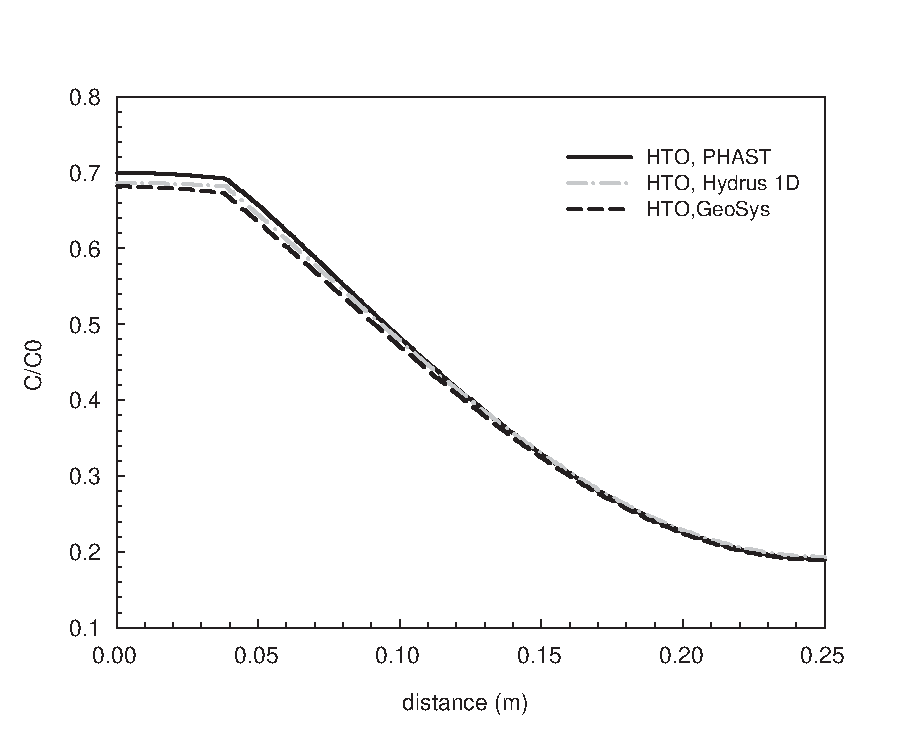
\includegraphics[width=0.8\textwidth]{PART_II/C/fig510.EPS}
\caption{Concentration distributions after 300~d}
\label{fig510}
\end{figure}

\subsubsection{Results}

In Figure \ref{fig510} you can find the concentration distributions over the width of 0.25~m after a simulation time of 300 days that were calculated by means of OGS, PHAST and Hydrus 1D (Bahr, 2007 \cite{Bahr:2007}). The numerical results accord well to each other. Thus, the comparison shows that the diffusion process can be well reproduced by the use of an axisymmetric numerical model.

%----------
\subsection{Anisotropy}

\subsubsection{Definition}

The aim of this example is to simulate the transport of a tracer by molecular diffusion in an anisotropic porous medium. The side length of the square numerical model is 1~m. At the left corner at the bottom of the model a constant concentration is diffusing into the calculation area. Diffusion is the only process for tracer transport, there are no pressure differences in the whole area. Because of the anisotropy of the soil material the tracer has to diffuse much faster in x-direction than in vertical direction. This has to be evaluated by comparing the concentration distributions in both directions.

As initial condition the pressure and tracer concentration were set to 0 in the whole area. At the left corner at the bottom of the model a concentration relation c/c$_0$ of 1 is specified along two polylines of the length of 0.3~m. The boundary conditions correspond to the initial conditions. The calculation model includes 736 triangular elements and 409 nodes. Table \ref{tab55} shows the used parameters for the simulation. As the porous medium is assumed to be anisotropic, which influences diffusion, the value for tortuosity is set equal to 1 in x-direction and 0.1 in y-direction.

\begin{table}[h]%[tab-ldhp]
\begin{center}
\begin{tabular}{llrr}
\toprule
Symbol & Parameter & Value & Unit \\
\midrule
$\Phi$ & Porosity & 0.4 & -- \\
$K$ & Permeability & 1.0$\cdot 10^{-15}$ & m$^2$ \\
$\rho$ & Density water & 1000 & kg/m$^{-3}$  \\		
$\eta$ & Viscosity water & 0.001 & Pa$\cdot$ s \\
$\alpha_T$ & Dispersion length & 10.0 & m \\
D$_a$ & Diffusion coefficient & 6.0$\cdot 10^{-10}$ & m$^2$/s  \\
\bottomrule
\end{tabular}
\caption{Model parameters}
\label{tab55}
\end{center}
\end{table}

The calculation is made for 30 time steps with a length of 1$\cdot$10$^7$ seconds. The calculation model is sketched in Figure \ref{fig511}.

\begin{figure}[htbp]
\centering
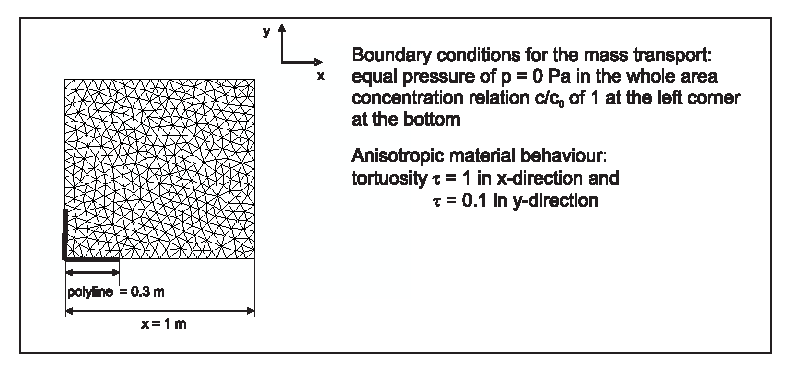
\includegraphics[width=0.9\textwidth]{PART_II/C/fig511.eps}
\caption{Benchmark definition}
\label{fig511}
\end{figure}

%\subsubsection*{Evaluation method}

As the process of diffusion is dependent on the actual concentration in the porous medium and on the point in time, an analytical solution for the present calculation model is not possible. Therefore, the results of the numerical simulation are solely evaluated in a qualitative way by comparing the concentration distributions in horizontal and vertical direction.

\begin{figure}[htbp]
\centering
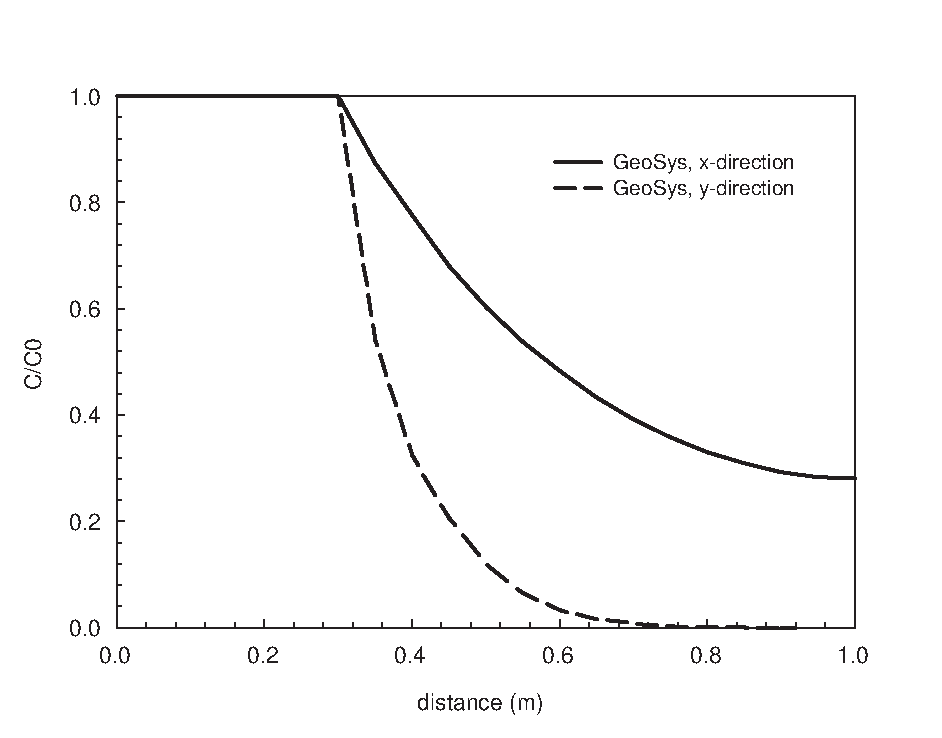
\includegraphics[width=0.8\textwidth]{PART_II/C/fig512.EPS}
\caption{Concentration distributions in x- and y-direction}
\label{fig512}
\end{figure}

\subsubsection{Results}

In Figure \ref{fig512} you can find the concentration distributions over the model side length of 1~m in x- and y-direction, respectively, after a simulation time of 1$\cdot$10$^8$ seconds. Assuming a small tortuosity of 0.1, the component is not yet transported over the whole transport length of 1~m in vertical direction, while in horizontal direction the concentration relation equals approximately 0.3 at the opposite border of the model. The shown trend in the change of diffusion velocity by assuming different tortuosities in x- and y-direction in order to specify anisotropic material behaviour for molecular diffusion has a comprehensible characteristic.
